\section{Graphs}

A \textbf{graph} is a data structure made up of \textbf{nodes} connected by \textbf{pointers}.
Graphs are used to model relationships between entities, such as:
\begin{itemize}
  \item Social networks (one person follows another)
  \item Maps (one city connected to another)
  \item Dependencies (one task must be completed before another)
\end{itemize}

\subsection{Graph Terminology}

In graphs:
\begin{itemize}
  \item Nodes are called \textbf{vertices}
  \item Pointers connecting nodes are called \textbf{edges}
\end{itemize}

Unlike trees and linked lists, graphs have \textbf{no restrictions} on how nodes are connected:
\begin{itemize}
  \item A node can have any number of edges
  \item Cycles are allowed
  \item Nodes don't need to be connected at all
\end{itemize}

The only restriction is the maximum number of edges:
\[
E \leq V^2
\]
This is because every vertex can have an edge pointed to every other vertex \textbf{plus itself}, leading to a maximum of $V^2$ edges. A graph with $V$ vertices and $V^2$ edges is called a \textbf{complete graph}.

\subsection{Directed vs Undirected Graphs}

\textbf{Directed Graph:}
Edges have a direction. An edge from $A$ to $B$ does \textbf{not} imply an edge from $B$ to $A$.

\begin{center}
\begin{tikzpicture}[
  >=Stealth,
  every node/.style={circle, draw, minimum size=10mm},
  edge/.style={->, thick}
]
\node (A) at (0,0) {A};
\node (B) at (3,0) {B};
\node (C) at (1.5,-2) {C};

\draw[edge] (A) -- (B);
\draw[edge] (B) -- (C);
\draw[edge] (C) -- (A);
\end{tikzpicture}

{\small Directed graph: $C \to A$ exists, but $A \to C$ does not}
\end{center}

Trees and linked lists are examples of directed graphs (pointers like \texttt{prev}, \texttt{next}, \texttt{left}, \texttt{right}).

\textbf{Undirected Graph:}
Edges have no direction. If there's an edge between $A$ and $B$, you can traverse in both directions.

\begin{center}
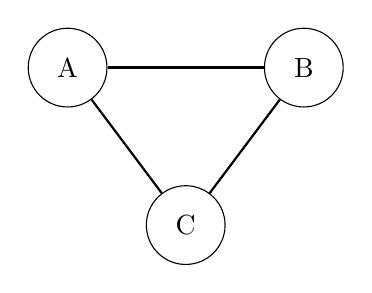
\begin{tikzpicture}[
  every node/.style={circle, draw, minimum size=10mm},
  edge/.style={-, thick}
]
\node (A) at (0,0) {A};
\node (B) at (3,0) {B};
\node (C) at (1.5,-2) {C};

\draw[edge] (A) -- (B);
\draw[edge] (B) -- (C);
\draw[edge] (C) -- (A);
\end{tikzpicture}

{\small Undirected graph: can traverse A--C in both directions}
\end{center}

\subsection{Matrix (Grid)}

Graphs can be represented using different data structures. The first representation is a Matrix.

A \textbf{matrix} is a 2D array where:
\begin{itemize}
  \item \texttt{0} represents a free cell (vertex)
  \item \texttt{1} represents a blocked cell
\end{itemize}

\begin{verbatim}
int[][] grid = {{0, 0, 0, 0},
                {1, 1, 0, 0},
                {0, 0, 0, 1},
                {0, 1, 0, 0}};
\end{verbatim}

To traverse the graph, we move \textbf{up, down, left, right} between adjacent 0s. Connected 0s form \textbf{connected components}.

\begin{center}
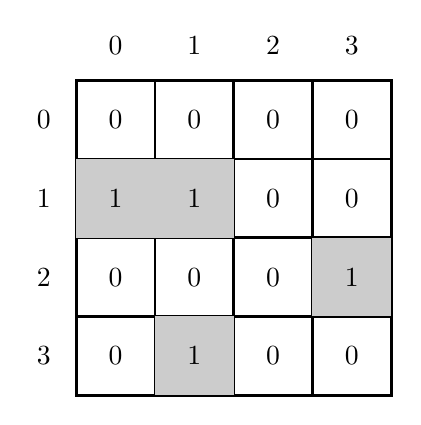
\begin{tikzpicture}[x=1cm,y=1cm]
  \def\cellW{1.0}
  \def\H{1.0}
  
  % Draw grid
  \foreach \row in {0,...,3} {
    \foreach \col in {0,...,3} {
      \draw[line width=1pt] ({\col*\cellW},{-\row*\H}) rectangle ({(\col+1)*\cellW},{(-\row-1)*\H});
    }
  }
  
  % Fill blocked cells (1s)
  \fill[gray!40] ({0*\cellW},{-1*\H}) rectangle ({1*\cellW},{-2*\H}); % [1][0]
  \fill[gray!40] ({1*\cellW},{-1*\H}) rectangle ({2*\cellW},{-2*\H}); % [1][1]
  \fill[gray!40] ({3*\cellW},{-2*\H}) rectangle ({4*\cellW},{-3*\H}); % [2][3]
  \fill[gray!40] ({1*\cellW},{-3*\H}) rectangle ({2*\cellW},{-4*\H}); % [3][1]
  
  % Add values
  \node at ({0.5*\cellW},{-0.5*\H}) {0};
  \node at ({1.5*\cellW},{-0.5*\H}) {0};
  \node at ({2.5*\cellW},{-0.5*\H}) {0};
  \node at ({3.5*\cellW},{-0.5*\H}) {0};
  
  \node at ({0.5*\cellW},{-1.5*\H}) {1};
  \node at ({1.5*\cellW},{-1.5*\H}) {1};
  \node at ({2.5*\cellW},{-1.5*\H}) {0};
  \node at ({3.5*\cellW},{-1.5*\H}) {0};
  
  \node at ({0.5*\cellW},{-2.5*\H}) {0};
  \node at ({1.5*\cellW},{-2.5*\H}) {0};
  \node at ({2.5*\cellW},{-2.5*\H}) {0};
  \node at ({3.5*\cellW},{-2.5*\H}) {1};
  
  \node at ({0.5*\cellW},{-3.5*\H}) {0};
  \node at ({1.5*\cellW},{-3.5*\H}) {1};
  \node at ({2.5*\cellW},{-3.5*\H}) {0};
  \node at ({3.5*\cellW},{-3.5*\H}) {0};
  
  % Row/column labels
  \node[anchor=east] at (-0.2,-0.5) {0};
  \node[anchor=east] at (-0.2,-1.5) {1};
  \node[anchor=east] at (-0.2,-2.5) {2};
  \node[anchor=east] at (-0.2,-3.5) {3};
  
  \node[anchor=south] at (0.5,0.2) {0};
  \node[anchor=south] at (1.5,0.2) {1};
  \node[anchor=south] at (2.5,0.2) {2};
  \node[anchor=south] at (3.5,0.2) {3};
\end{tikzpicture}
\end{center}

\textbf{Space Complexity:} $O(n \cdot m)$ where $n$ is rows and $m$ is columns.

\subsection{Adjacency Matrix}

An \textbf{adjacency matrix} is another representation, and is a 2D array where indices represent vertices:
\begin{itemize}
  \item \texttt{adjMatrix[v1][v2] = 1} means an edge exists from \texttt{v1} to \texttt{v2}
  \item \texttt{adjMatrix[v1][v2] = 0} means no edge exists from \texttt{v1} to \texttt{v2}
\end{itemize}

\begin{verbatim}
int[][] adjMatrix = {{0, 0, 0, 0},
                     {1, 1, 0, 0},
                     {0, 0, 0, 1},
                     {0, 1, 0, 0}};
\end{verbatim}

\begin{center}
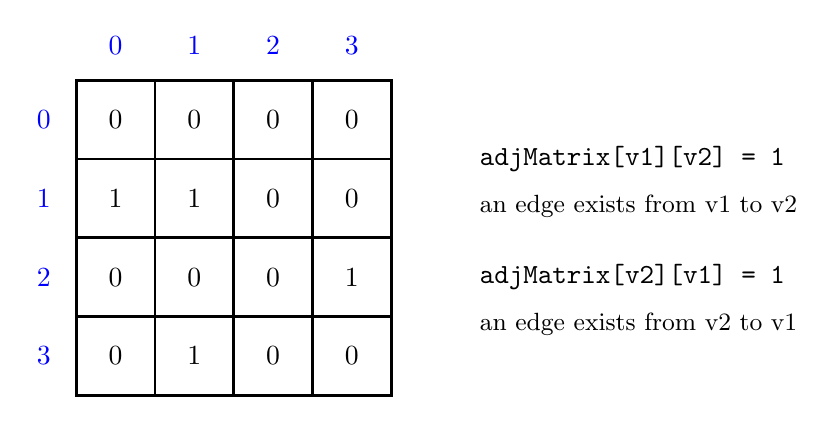
\begin{tikzpicture}[x=1cm,y=1cm]
  \def\cellW{1.0}
  \def\H{1.0}
  
  % Draw grid
  \foreach \row in {0,...,3} {
    \foreach \col in {0,...,3} {
      \draw[line width=1pt] ({\col*\cellW},{-\row*\H}) rectangle ({(\col+1)*\cellW},{(-\row-1)*\H});
    }
  }
  
  % Add values - row 0
  \node at ({0.5*\cellW},{-0.5*\H}) {0};
  \node at ({1.5*\cellW},{-0.5*\H}) {0};
  \node at ({2.5*\cellW},{-0.5*\H}) {0};
  \node at ({3.5*\cellW},{-0.5*\H}) {0};
  
  % Row 1
  \node at ({0.5*\cellW},{-1.5*\H}) {1};
  \node at ({1.5*\cellW},{-1.5*\H}) {1};
  \node at ({2.5*\cellW},{-1.5*\H}) {0};
  \node at ({3.5*\cellW},{-1.5*\H}) {0};
  
  % Row 2
  \node at ({0.5*\cellW},{-2.5*\H}) {0};
  \node at ({1.5*\cellW},{-2.5*\H}) {0};
  \node at ({2.5*\cellW},{-2.5*\H}) {0};
  \node at ({3.5*\cellW},{-2.5*\H}) {1};
  
  % Row 3
  \node at ({0.5*\cellW},{-3.5*\H}) {0};
  \node at ({1.5*\cellW},{-3.5*\H}) {1};
  \node at ({2.5*\cellW},{-3.5*\H}) {0};
  \node at ({3.5*\cellW},{-3.5*\H}) {0};
  
  % Row/column labels
  \node[anchor=east,blue] at (-0.2,-0.5) {0};
  \node[anchor=east,blue] at (-0.2,-1.5) {1};
  \node[anchor=east,blue] at (-0.2,-2.5) {2};
  \node[anchor=east,blue] at (-0.2,-3.5) {3};
  
  \node[anchor=south,blue] at (0.5,0.2) {0};
  \node[anchor=south,blue] at (1.5,0.2) {1};
  \node[anchor=south,blue] at (2.5,0.2) {2};
  \node[anchor=south,blue] at (3.5,0.2) {3};
  
  % Annotations
  \node[anchor=west] at (5,-1) {\texttt{adjMatrix[v1][v2] = 1}};
  \node[anchor=west] at (5,-1.6) {\small an edge exists from v1 to v2};
  
  \node[anchor=west] at (5,-2.5) {\texttt{adjMatrix[v2][v1] = 1}};
  \node[anchor=west] at (5,-3.1) {\small an edge exists from v2 to v1};
\end{tikzpicture}
\end{center}

From the matrix above:
\begin{itemize}
  \item \texttt{adjMatrix[1][0] = 1}: edge from vertex 1 to vertex 0
  \item \texttt{adjMatrix[1][1] = 1}: edge from vertex 1 to itself (self-loop)
  \item \texttt{adjMatrix[2][3] = 1}: edge from vertex 2 to vertex 3
  \item \texttt{adjMatrix[3][1] = 1}: edge from vertex 3 to vertex 1
\end{itemize}

\begin{center}
\begin{tikzpicture}[
  >=Stealth,
  every node/.style={circle, draw, minimum size=10mm},
  edge/.style={->, thick}
]
\node (0) at (0,0) {0};
\node (1) at (3,0) {1};
\node (2) at (3,-3) {2};
\node (3) at (0,-3) {3};

\draw[edge] (1) -- (0);
\draw[edge] (1) to [out=45,in=135,looseness=5] (1); % self-loop
\draw[edge] (2) -- (3);
\draw[edge] (3) -- (1);
\end{tikzpicture}

{\small Graph represented by the adjacency matrix}
\end{center}

\textbf{Drawback:} If the graph has few edges, most of the matrix is wasted storing 0s.

\textbf{Space Complexity:} $O(V^2)$ where $V$ is the number of vertices.

\subsection{Adjacency List}

Another common way to represent a graph is with an \textbf{adjacency list}, where each vertex maps to a list of its neighboring vertices. An adjacency list is more efficiently stored as a \textbf{List} or  \textbf{HashMap}, where each key is a vertex and the value is the list of its neighbors, allowing $O(1)$ average-time lookups. For example, given the following directed graph:

\begin{center}
\begin{tikzpicture}[
  >=Stealth,
  every node/.style={circle, draw, minimum size=10mm},
  edge/.style={->, thick}
]
\node (A) at (0,0) {A};
\node (B) at (0,-2) {B};
\node (C) at (0,-4) {C};
\node (D) at (3,0) {D};
\node (E) at (3,-2.5) {E};

\draw[edge] (A) -- (B);
\draw[edge] (B) -- (C);
\draw[edge] (B) -- (E);
\draw[edge] (C) -- (E);
\draw[edge] (E) -- (D);
\end{tikzpicture}
\end{center}
The adjacency list equivalent is:

\begin{center}
\begin{tikzpicture}[x=1cm,y=1cm,>=Stealth]
  % Node boxes
  \foreach \i/\val in {0/A, 1/B, 2/C, 3/D, 4/E} {
    % Node value box
    \draw[line width=1pt] (0,{-\i*1.2}) rectangle (1,{-\i*1.2-0.8});
    \node at (0.5,{-\i*1.2-0.4}) {\val};
    
    % Arrow to neighbors
    \draw[->,thick] (1,{-\i*1.2-0.4}) -- (1.5,{-\i*1.2-0.4});
  }
  
  % Neighbor lists
  \node[anchor=west] at (1.6,-0.4) {[B]};
  \node[anchor=west] at (1.6,-1.6) {[C, E]};
  \node[anchor=west] at (1.6,-2.8) {[E]};
  \node[anchor=west] at (1.6,-4.0) {[ ]};
  \node[anchor=west] at (1.6,-5.2) {[D]};
  
  % Labels
  \node[anchor=east] at (-0.2,-0.4) {vertex A:};
  \node[anchor=east] at (-0.2,-1.6) {vertex B:};
  \node[anchor=east] at (-0.2,-2.8) {vertex C:};
  \node[anchor=east] at (-0.2,-4.0) {vertex D:};
  \node[anchor=east] at (-0.2,-5.2) {vertex E:};
\end{tikzpicture}
\end{center}

\subsubsection{DFS (contains a path)}

We can traverse an adjacency list using \textbf{Depth-First Search (DFS)}. The algorithm marks each vertex as visited and records the edge used to reach it, allowing us to reconstruct the path from any vertex back to the source.

\textbf{Example: DFS from A (source = A)}

\textbf{Step 1:} Mark A as visited. Check neighbors: B is unmarked, set \texttt{edgeTo[B] = A}. Visit B.

\begin{center}
\begin{tikzpicture}[
  >=Stealth,
  every node/.style={circle, draw, minimum size=10mm},
  edge/.style={->, thick},
  highlight/.style={circle, draw, fill=blue!20, minimum size=10mm},
  hedge/.style={->, thick, blue}
]
\node[highlight] (A) at (0,0) {A};
\node (B) at (0,-2) {B};
\node (C) at (0,-4) {C};
\node (D) at (3,0) {D};
\node (E) at (3,-2.5) {E};

\draw[hedge] (A) -- (B);
\draw[edge] (B) -- (C);
\draw[edge] (B) -- (E);
\draw[edge] (C) -- (E);
\draw[edge] (E) -- (D);
\end{tikzpicture}

{\small marked = \{A\} \quad edgeTo[B] = A}
\end{center}

\textbf{Step 2:} Mark B as visited. Check neighbors: C is unmarked, set \texttt{edgeTo[C] = B}. Visit C.

\begin{center}
\begin{tikzpicture}[
  >=Stealth,
  every node/.style={circle, draw, minimum size=10mm},
  edge/.style={->, thick},
  highlight/.style={circle, draw, fill=blue!20, minimum size=10mm},
  hedge/.style={->, thick, blue}
]
\node[highlight] (A) at (0,0) {A};
\node[highlight] (B) at (0,-2) {B};
\node (C) at (0,-4) {C};
\node (D) at (3,0) {D};
\node (E) at (3,-2.5) {E};

\draw[hedge] (A) -- (B);
\draw[hedge] (B) -- (C);
\draw[edge] (B) -- (E);
\draw[edge] (C) -- (E);
\draw[edge] (E) -- (D);
\end{tikzpicture}

{\small marked = \{A, B\} \quad edgeTo[C] = B}
\end{center}

\textbf{Step 3:} Mark C as visited. Check neighbors: E is unmarked, set \texttt{edgeTo[E] = C}. Visit E.

\begin{center}
\begin{tikzpicture}[
  >=Stealth,
  every node/.style={circle, draw, minimum size=10mm},
  edge/.style={->, thick},
  highlight/.style={circle, draw, fill=blue!20, minimum size=10mm},
  hedge/.style={->, thick, blue}
]
\node[highlight] (A) at (0,0) {A};
\node[highlight] (B) at (0,-2) {B};
\node[highlight] (C) at (0,-4) {C};
\node (D) at (3,0) {D};
\node (E) at (3,-2.5) {E};

\draw[hedge] (A) -- (B);
\draw[hedge] (B) -- (C);
\draw[edge] (B) -- (E);
\draw[hedge] (C) -- (E);
\draw[edge] (E) -- (D);
\end{tikzpicture}

{\small marked = \{A, B, C\} \quad edgeTo[E] = C}
\end{center}

\textbf{Step 4:} Mark E as visited. Check neighbors: D is unmarked, set \texttt{edgeTo[D] = E}. Visit D.

\begin{center}
\begin{tikzpicture}[
  >=Stealth,
  every node/.style={circle, draw, minimum size=10mm},
  edge/.style={->, thick},
  highlight/.style={circle, draw, fill=blue!20, minimum size=10mm},
  hedge/.style={->, thick, blue}
]
\node[highlight] (A) at (0,0) {A};
\node[highlight] (B) at (0,-2) {B};
\node[highlight] (C) at (0,-4) {C};
\node (D) at (3,0) {D};
\node[highlight] (E) at (3,-2.5) {E};

\draw[hedge] (A) -- (B);
\draw[hedge] (B) -- (C);
\draw[edge] (B) -- (E);
\draw[hedge] (C) -- (E);
\draw[hedge] (E) -- (D);
\end{tikzpicture}

{\small marked = \{A, B, C, E\} \quad edgeTo[D] = E}
\end{center}

\textbf{Step 5:} Mark D as visited. D has no unmarked neighbors. Backtrack to E, then B. B's second neighbor E is already marked. Done.

\begin{center}
\begin{tikzpicture}[
  >=Stealth,
  every node/.style={circle, draw, minimum size=10mm},
  edge/.style={->, thick},
  highlight/.style={circle, draw, fill=blue!20, minimum size=10mm},
  hedge/.style={->, thick, blue}
]
\node[highlight] (A) at (0,0) {A};
\node[highlight] (B) at (0,-2) {B};
\node[highlight] (C) at (0,-4) {C};
\node[highlight] (D) at (3,0) {D};
\node[highlight] (E) at (3,-2.5) {E};

\draw[hedge] (A) -- (B);
\draw[hedge] (B) -- (C);
\draw[edge] (B) -- (E);
\draw[hedge] (C) -- (E);
\draw[hedge] (E) -- (D);
\end{tikzpicture}

{\small All vertices marked.}
\end{center}

Using \texttt{edgeTo}, we can reconstruct the path from A to any vertex. For example, the path from A to D: follow \texttt{edgeTo[D] = E}, \texttt{edgeTo[E] = C}, \texttt{edgeTo[C] = B}, \texttt{edgeTo[B] = A}, giving us $A \rightarrow B \rightarrow C \rightarrow E \rightarrow D$.

To implement this, we use the following code:
\begin{verbatim}
public class DepthFirstPaths {
    Set<String> marked;
    Map<String, String> edgeTo;
    String s;

    public DepthFirstPaths(Graph G, String s) {
        marked = new HashSet<>();
        edgeTo = new HashMap<>();
        this.s = s;
        dfs(G, s);
    }

    private void dfs(Graph G, String v) {
        marked.add(v);
        for (String w : G.adj(v)) {
            if (!marked.contains(w)) {
                edgeTo.put(w, v);
                dfs(G, w);
            }
        }
    }
}
\end{verbatim}


\textbf{Time Complexity:} The time complexity for this DFS algorithm is
\[
O(V + E),
\]
as each vertex is visited once, and each edge is checked once for unvisited vertices.


\begin{itemize}
  \item \texttt{marked[v]}: whether vertex \texttt{v} has been visited
  \item \texttt{edgeTo[w] = v}: vertex \texttt{v} was used to reach \texttt{w}
  \item \texttt{G.adj(v)}: the adjacency list of vertex \texttt{v}
\end{itemize}

\subsubsection{DFS: number of unique paths}
We can use DFS to find the total number of unique paths to a targe node. 

\textbf{Example: count all unique paths from A to E}

\textbf{Step 1:} Start at A. A $\neq$ E, add A to visited. Visit neighbor B.

\begin{center}
\begin{tikzpicture}[
  >=Stealth,
  every node/.style={circle, draw, minimum size=10mm},
  edge/.style={->, thick},
  highlight/.style={circle, draw, fill=blue!20, minimum size=10mm},
  hedge/.style={->, thick, blue}
]
\node[highlight] (A) at (0,0) {A};
\node (B) at (0,-2) {B};
\node (C) at (0,-4) {C};
\node (D) at (3,0) {D};
\node (E) at (3,-2.5) {E};

\draw[hedge] (A) -- (B);
\draw[edge] (B) -- (C);
\draw[edge] (B) -- (E);
\draw[edge] (C) -- (E);
\draw[edge] (E) -- (D);
\end{tikzpicture}

{\small visited = \{A\}}
\end{center}

\textbf{Step 2:} At B. B $\neq$ E, add B to visited. Visit first neighbor C.

\begin{center}
\begin{tikzpicture}[
  >=Stealth,
  every node/.style={circle, draw, minimum size=10mm},
  edge/.style={->, thick},
  highlight/.style={circle, draw, fill=blue!20, minimum size=10mm},
  hedge/.style={->, thick, blue}
]
\node[highlight] (A) at (0,0) {A};
\node[highlight] (B) at (0,-2) {B};
\node (C) at (0,-4) {C};
\node (D) at (3,0) {D};
\node (E) at (3,-2.5) {E};

\draw[hedge] (A) -- (B);
\draw[hedge] (B) -- (C);
\draw[edge] (B) -- (E);
\draw[edge] (C) -- (E);
\draw[edge] (E) -- (D);
\end{tikzpicture}

{\small visited = \{A, B\}}
\end{center}

\textbf{Step 3:} At C. C $\neq$ E, add C to visited. Visit neighbor E.

\begin{center}
\begin{tikzpicture}[
  >=Stealth,
  every node/.style={circle, draw, minimum size=10mm},
  edge/.style={->, thick},
  highlight/.style={circle, draw, fill=blue!20, minimum size=10mm},
  hedge/.style={->, thick, blue}
]
\node[highlight] (A) at (0,0) {A};
\node[highlight] (B) at (0,-2) {B};
\node[highlight] (C) at (0,-4) {C};
\node (D) at (3,0) {D};
\node (E) at (3,-2.5) {E};

\draw[hedge] (A) -- (B);
\draw[hedge] (B) -- (C);
\draw[edge] (B) -- (E);
\draw[hedge] (C) -- (E);
\draw[edge] (E) -- (D);
\end{tikzpicture}

{\small visited = \{A, B, C\}}
\end{center}

\textbf{Step 4:} At E. E == target: path found! Count = 1. Backtrack: remove C from visited.

\begin{center}
\begin{tikzpicture}[
  >=Stealth,
  every node/.style={circle, draw, minimum size=10mm},
  edge/.style={->, thick},
  highlight/.style={circle, draw, fill=blue!20, minimum size=10mm},
  found/.style={circle, draw, fill=green!20, minimum size=10mm},
  hedge/.style={->, thick, blue}
]
\node[highlight] (A) at (0,0) {A};
\node[highlight] (B) at (0,-2) {B};
\node[highlight] (C) at (0,-4) {C};
\node (D) at (3,0) {D};
\node[found] (E) at (3,-2.5) {E};

\draw[hedge] (A) -- (B);
\draw[hedge] (B) -- (C);
\draw[edge] (B) -- (E);
\draw[hedge] (C) -- (E);
\draw[edge] (E) -- (D);
\end{tikzpicture}

{\small Path 1: $A \rightarrow B \rightarrow C \rightarrow E$ \quad visited = \{A, B\}}
\end{center}

\textbf{Step 5:} Back at B. C already explored, visit second neighbor E.

\begin{center}
\begin{tikzpicture}[
  >=Stealth,
  every node/.style={circle, draw, minimum size=10mm},
  edge/.style={->, thick},
  highlight/.style={circle, draw, fill=blue!20, minimum size=10mm},
  hedge/.style={->, thick, blue}
]
\node[highlight] (A) at (0,0) {A};
\node[highlight] (B) at (0,-2) {B};
\node (C) at (0,-4) {C};
\node (D) at (3,0) {D};
\node (E) at (3,-2.5) {E};

\draw[hedge] (A) -- (B);
\draw[edge] (B) -- (C);
\draw[hedge] (B) -- (E);
\draw[edge] (C) -- (E);
\draw[edge] (E) -- (D);
\end{tikzpicture}

{\small visited = \{A, B\}}
\end{center}

\textbf{Step 6:} At E. E == target: path found! Count = 2. Backtrack: remove B, A. All neighbors exhausted.

\begin{center}
\begin{tikzpicture}[
  >=Stealth,
  every node/.style={circle, draw, minimum size=10mm},
  edge/.style={->, thick},
  highlight/.style={circle, draw, fill=blue!20, minimum size=10mm},
  found/.style={circle, draw, fill=green!20, minimum size=10mm},
  hedge/.style={->, thick, blue}
]
\node[highlight] (A) at (0,0) {A};
\node[highlight] (B) at (0,-2) {B};
\node (C) at (0,-4) {C};
\node (D) at (3,0) {D};
\node[found] (E) at (3,-2.5) {E};

\draw[hedge] (A) -- (B);
\draw[edge] (B) -- (C);
\draw[hedge] (B) -- (E);
\draw[edge] (C) -- (E);
\draw[edge] (E) -- (D);
\end{tikzpicture}

{\small Path 2: $A \rightarrow B \rightarrow E$ \quad visited = \{\}}
\end{center}

\textbf{Result:} \texttt{dfs("A", "E", adjList, new HashSet<>())} returns \textbf{2} unique paths.

To implement this, we use the following code:

\begin{verbatim}
public class CountPaths {
    Map<String, List<String>> adjList;
    Set<String> visited;

    public CountPaths(Map<String, List<String>> adjList) {
        this.adjList = adjList;
        this.visited = new HashSet<>();
    }

    public int dfs(String node, String target) {
        if (visited.contains(node)) return 0;
        if (node.equals(target)) return 1;

        int count = 0;
        visited.add(node);
        for (String neighbor : adjList.get(node)) {
            count += dfs(neighbor, target);
        }
        visited.remove(node);
        return count;
    }
}
\end{verbatim}

\textbf{Time Complexity:} 
The worst case of this algorithm is:
\[
O(V!)
\]
in a complete graph, since at each step we have one fewer unvisited node to chose from $(V-1) \times (V-2) \times \cdots \times 1$.

\subsubsection{BFS (Shortest Path)}

We can also traverse an adjacency list using \textbf{Breadth-First Search (BFS)}. Unlike DFS, BFS explores vertices \textbf{level by level}, making it ideal for finding the \textbf{shortest path} from a source to a target.

BFS uses a \textbf{queue (FIFO)} because nodes are processed in the order they are discovered.

\textbf{Example: shortest path from A to E}

\textbf{Step 1:} Start at A. Add A to queue and visited. Process level 0: A $\neq$ E. Add neighbor B to queue.

\begin{center}
\begin{tikzpicture}[
  >=Stealth,
  every node/.style={circle, draw, minimum size=10mm},
  edge/.style={->, thick},
  highlight/.style={circle, draw, fill=blue!20, minimum size=10mm},
  hedge/.style={->, thick, blue}
]
\node[highlight] (A) at (0,0) {A};
\node (B) at (0,-2) {B};
\node (C) at (0,-4) {C};
\node (D) at (3,0) {D};
\node (E) at (3,-2.5) {E};

\draw[edge] (A) -- (B);
\draw[edge] (B) -- (C);
\draw[edge] (B) -- (E);
\draw[edge] (C) -- (E);
\draw[edge] (E) -- (D);
\end{tikzpicture}

{\small queue = [B] \quad visited = \{A, B\} \quad length = 0}
\end{center}

\textbf{Step 2:} Process level 1: B $\neq$ E. Add neighbors C and E to queue.

\begin{center}
\begin{tikzpicture}[
  >=Stealth,
  every node/.style={circle, draw, minimum size=10mm},
  edge/.style={->, thick},
  highlight/.style={circle, draw, fill=blue!20, minimum size=10mm},
  hedge/.style={->, thick, blue}
]
\node[highlight] (A) at (0,0) {A};
\node[highlight] (B) at (0,-2) {B};
\node (C) at (0,-4) {C};
\node (D) at (3,0) {D};
\node (E) at (3,-2.5) {E};

\draw[hedge] (A) -- (B);
\draw[edge] (B) -- (C);
\draw[edge] (B) -- (E);
\draw[edge] (C) -- (E);
\draw[edge] (E) -- (D);
\end{tikzpicture}

{\small queue = [C, E] \quad visited = \{A, B, C, E\} \quad length = 1}
\end{center}

\textbf{Step 3:} Process level 2: first in queue is C, C $\neq$ E. 

Next in queue is E, E == target, return length = 2.

\begin{center}
\begin{tikzpicture}[
  >=Stealth,
  every node/.style={circle, draw, minimum size=10mm},
  edge/.style={->, thick},
  highlight/.style={circle, draw, fill=blue!20, minimum size=10mm},
  found/.style={circle, draw, fill=green!20, minimum size=10mm},
  hedge/.style={->, thick, blue}
]
\node[highlight] (A) at (0,0) {A};
\node[highlight] (B) at (0,-2) {B};
\node[highlight] (C) at (0,-4) {C};
\node (D) at (3,0) {D};
\node[found] (E) at (3,-2.5) {E};

\draw[hedge] (A) -- (B);
\draw[hedge] (B) -- (C);
\draw[hedge] (B) -- (E);
\draw[edge] (C) -- (E);
\draw[edge] (E) -- (D);
\end{tikzpicture}

{\small Shortest path: $A \rightarrow B \rightarrow E$ \quad length = 2}
\end{center}

\textbf{Result:} \texttt{bfs("A", "E")} returns \textbf{2}, the shortest path from A to E.

To implement this, we use the following code:

\begin{verbatim}
public class ShortestPath {
    Map<String, List<String>> adjList;
    Set<String> visited;

    public ShortestPath(Map<String, List<String>> adjList) {
        this.adjList = adjList;
        this.visited = new HashSet<>();
    }

    public int bfs(String node, String target) {
        int length = 0;
        visited.add(node);
        Queue<String> queue = new LinkedList<>();
        queue.add(node);

        while (!queue.isEmpty()) {
            int size = queue.size();
            for (int i = 0; i < size; i++) {
                String curr = queue.poll();
                if (curr.equals(target)) return length;

                for (String neighbor : adjList.get(curr)) {
                    if (!visited.contains(neighbor)) {
                        visited.add(neighbor);
                        queue.add(neighbor);
                    }
                }
            }
            length++;
        }
        return -1;
    }
}
\end{verbatim}

\begin{itemize}
  \item \texttt{visited}: tracks which vertices have been seen to avoid revisiting
  \item \texttt{queue}: processes vertices in FIFO order, ensuring level-by-level traversal
  \item \texttt{length}: increments after each level, tracking distance from source
\end{itemize}

\textbf{Time Complexity:} 
The time complexity for this BFS algorithm is
\[
O(V + E),
\]

as each vertex is visited once, and each edge is checked once for unvisited vertices.

\subsection{Summary}

\begin{center}
\begin{tabular}{|l|l|}
\hline
\textbf{Algorithm} & \textbf{Time Complexity} \\
\hline
DFS (path exists) & $O(V + E)$ \\
\hline
DFS (count unique paths) & $O(V!)$ \\
\hline
BFS (shortest path, unweighted) & $O(V + E)$ \\
\hline
\end{tabular}
\end{center}

\begin{center}
\begin{tabular}{|l|l|}
\hline
\textbf{Representation} & \textbf{Space Complexity} \\
\hline
Matrix (Grid) & $O(n \cdot m)$ \\
\hline
Adjacency Matrix & $O(V^2)$ \\
\hline
Adjacency List & $O(V + E)$ \\
\hline
\end{tabular}
\end{center}